\documentclass[12pt,letterpaper]{article}
\usepackage{graphicx,textcomp}
\usepackage{natbib}
\usepackage{setspace}
\usepackage{fullpage}
\usepackage{color}
\usepackage[reqno]{amsmath}
\usepackage{amsthm}
\usepackage{fancyvrb}
\usepackage{amssymb,enumerate}
\usepackage[all]{xy}
\usepackage{endnotes}
\usepackage{adjustbox}
\usepackage{lscape}
\newtheorem{com}{Comment}
\usepackage{float}
\usepackage{hyperref}
\newtheorem{lem} {Lemma}
\newtheorem{prop}{Proposition}
\newtheorem{thm}{Theorem}
\newtheorem{defn}{Definition}
\newtheorem{cor}{Corollary}
\usepackage{enumitem}

\newtheorem{obs}{Observation}
\usepackage[compact]{titlesec}
\usepackage{dcolumn}
\usepackage{tikz}
\usetikzlibrary{arrows}
\usepackage{multirow}
\usepackage{xcolor}
\newcolumntype{.}{D{.}{.}{-1}}
\newcolumntype{d}[1]{D{.}{.}{#1}}
\definecolor{light-gray}{gray}{0.65}
\usepackage{url}
\usepackage{listings}
\usepackage{color}

\definecolor{codegreen}{rgb}{0,0.6,0}
\definecolor{codegray}{rgb}{0.5,0.5,0.5}
\definecolor{codepurple}{rgb}{0.58,0,0.82}
\definecolor{backcolour}{rgb}{0.95,0.95,0.92}

\lstdefinestyle{mystyle}{
	backgroundcolor=\color{backcolour},   
	commentstyle=\color{codegreen},
	keywordstyle=\color{magenta},
	numberstyle=\tiny\color{codegray},
	stringstyle=\color{codepurple},
	basicstyle=\footnotesize,
	breakatwhitespace=false,         
	breaklines=true,                 
	captionpos=b,                    
	keepspaces=true,                 
	numbers=left,                    
	numbersep=5pt,                  
	showspaces=false,                
	showstringspaces=false,
	showtabs=false,                  
	tabsize=2
}
\lstset{style=mystyle}
\newcommand{\Sref}[1]{Section~\ref{#1}}
\newtheorem{hyp}{Hypothesis}

\title{Answer Key: Problem Set 3}
\date{Jeffrey Ziegler}
\author{Applied Stats/Quant Methods 1}

\begin{document}
	\maketitle
	
	\section*{Instructions}
	\begin{itemize}
		\item \textit{Please show your work! You may lose points by simply writing in the answer. If the problem requires you to execute commands in \texttt{R}, please include the code you used to get your answers. Please also include the \texttt{.R} file that contains your code. If you are not sure if work needs to be shown for a particular problem, please ask.}
		\item \textit{Your homework should be submitted electronically on GitHub in \texttt{.pdf} form.}
		\item \textit{This problem set is due before 23:59 on Monday November 11, 2024. No late assignments will be accepted.}

	\end{itemize}
	\vspace{.25cm}
	
	\noindent \emph{In this problem set, you will run several regressions and create an add variable plot (see the lecture slides) in \texttt{R} using the \texttt{incumbents\_subset.csv} dataset. Include all of your code.}
	
	\vspace{.5cm}
	\section*{Question 1}
	\vspace{.25cm}
	\noindent \emph{We are interested in knowing how the difference in campaign spending between incumbent and challenger affects the incumbent's vote share. }
	\begin{enumerate}
		\item \emph{Run a regression where the outcome variable is \texttt{voteshare} and the explanatory variable is \texttt{difflog}.	}\vspace{.25cm}
			\lstinputlisting[language=R, firstline=37, lastline=43]{PS3_answerKey.R}  
			\clearpage

\begin{table}
\begin{center}
	\caption{\footnotesize{Outcome variable is \texttt{voteshare} and the explanatory variable is \texttt{difflog}.}} %\vspace{.15cm}
	\label{table:coefficients}
\begin{tabular}{l c }
\hline
 & Model 1 \\
\hline
(Intercept) & $0.579^{***}$ \\
            & $(0.002)$     \\
difflog     & $0.042^{***}$ \\
            & $(0.001)$     \\
\hline
R$^2$       & 0.367         \\
Adj. R$^2$  & 0.367         \\
Num. obs.   & 3193          \\
RMSE        & 0.079         \\
\hline
\multicolumn{2}{l}{\scriptsize{$^{***}p<0.001$, $^{**}p<0.01$, $^*p<0.05$}}
\end{tabular}
\end{center}
\end{table}
		
\vspace{-1cm}
\noindent There is a positive and statistically reliable relationship between the amount of spending between the incumbent and challenger and the incumbent's vote share, such that a one unit increase in the logged difference in spending is associated with an average increase of 0.04 in the incumbent's vote share (4\%)	\vspace{.25cm}
		
		\item \emph{Make a scatterplot of the two variables and add the regression line. }	\vspace{.25cm}
		
					\lstinputlisting[language=R, firstline=47, lastline=49]{PS3_answerKey.R}  %\newpage
					
		\begin{figure}[b!]\centering
			\caption{\footnotesize Scatter plot of \texttt{difflog} and \texttt{voteshare}.}\vspace{-1cm}
			\label{fig:Q1_b}
			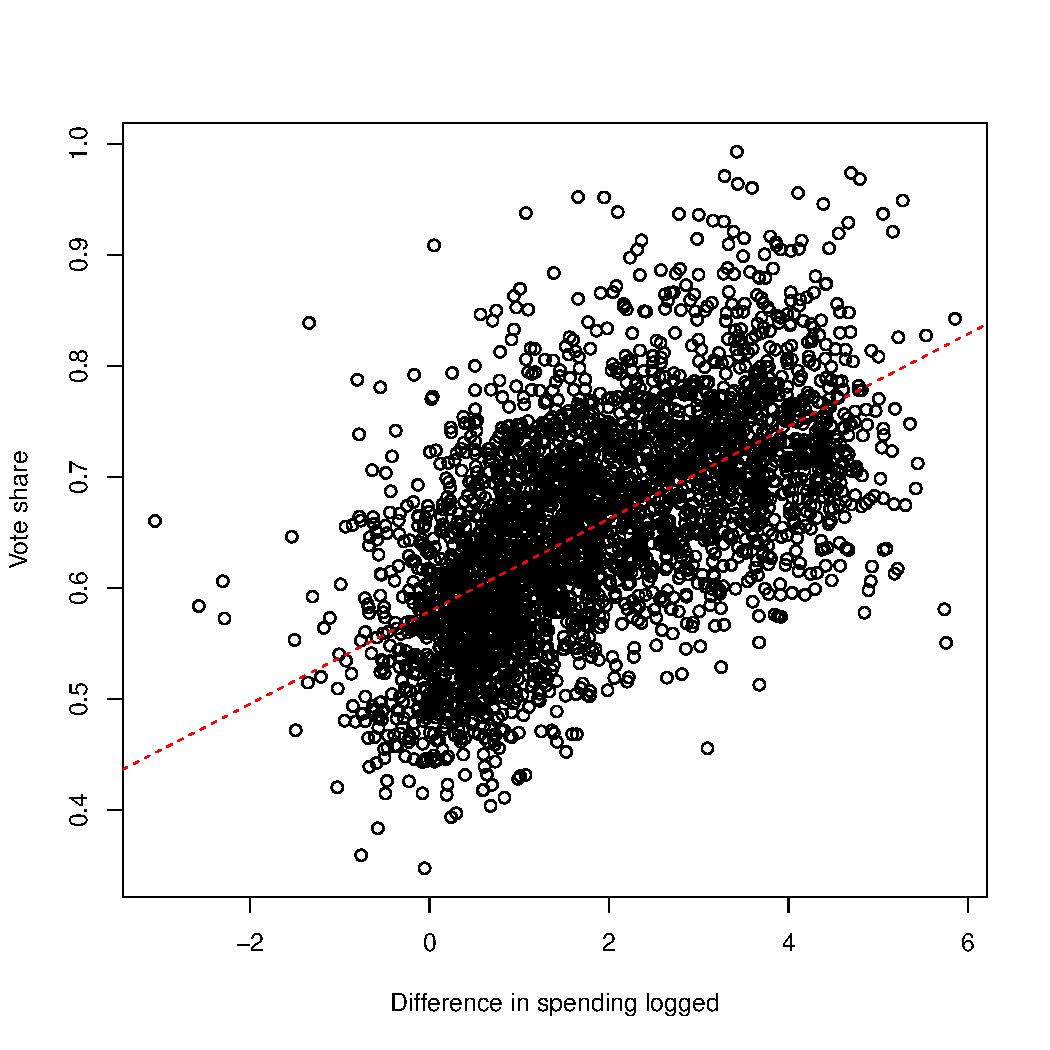
\includegraphics[width=.55\textwidth]{Q1_b.pdf}\\
		\end{figure}
	
\newpage
		\item \emph{Save the residuals of the model in a separate object.}	\vspace{.25cm}
							\lstinputlisting[language=R, firstline=53, lastline=53]{PS3_answerKey.R}  %\newpage
							
							\vspace{.25cm}
		\item \emph{Write the prediction equation.}\vspace{.25cm}
		
		\begin{align*}
		\hat{y} &= \hat{\beta_0} + \hat{\beta_1} \times  \text{difflog}\\
		voteshare &= 0.579 + 0.042 \times \text{difflog}
		\end{align*}
	\end{enumerate}
	
	\section*{Question 2}
	\noindent \emph{We are interested in knowing how the difference between incumbent and challenger's spending and the vote share of the presidential candidate of the incumbent's party are related.}	\vspace{.25cm}
	\begin{enumerate}
		\item \emph{Run a regression where the outcome variable is \texttt{presvote} and the explanatory variable is \texttt{difflog}.}
		
				\lstinputlisting[language=R, firstline=59, lastline=61]{PS3_answerKey.R}% \vspace{.25cm}
		
		\begin{table}[h!]
			\begin{center}
				\caption{\footnotesize{Outcome variable is \texttt{presvote} and the explanatory variable is \texttt{difflog}.}} %\vspace{.15cm}
			%	\label{table:coefficients}
				\begin{tabular}{l c }
					\hline
					& Model 1 \\
					\hline
				(Intercept) & $0.508^{***}$ \\
            & $(0.003)$     \\
difflog     & $0.024^{***}$ \\
            & $(0.001)$     \\
\hline
R$^2$       & 0.088         \\
Adj. R$^2$  & 0.088         \\
Num. obs.   & 3193          \\
RMSE        & 0.110         \\
					\hline
					\multicolumn{2}{l}{\scriptsize{$^{***}p<0.001$, $^{**}p<0.01$, $^*p<0.05$}}
				\end{tabular}
				
			\end{center}
		\end{table}
		
		%\vspace{.15cm}
		
		\noindent There is a positive and statistically reliable relationship between the amount of spending between the incumbent and challenger and the president vote share, such that a one unit increase in the logged difference in spending is associated with an average increase of 0.024 in the incumbent's vote share (2.4\%)	
		\newpage
		
		\item \emph{Make a scatterplot of the two variables and add the regression line. }	\vspace{.25cm}
		
						\lstinputlisting[language=R, firstline=65, lastline=67]{PS3_answerKey.R}  
		
		\begin{figure}[h!]\centering
			\caption{\footnotesize Scatter plot of \texttt{difflog} and \texttt{presshare}.}\vspace{-1cm}
			\label{fig:Q2_b}
			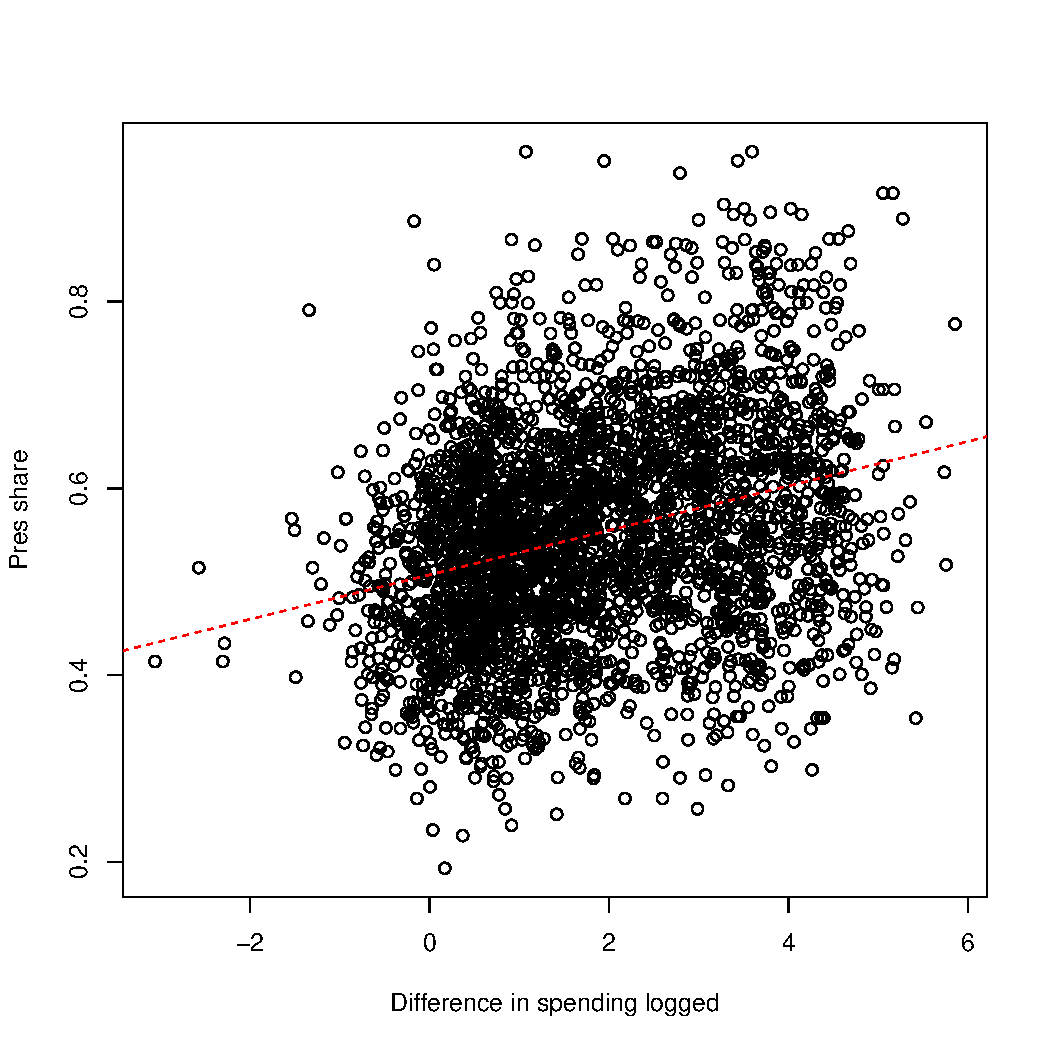
\includegraphics[width=.65\textwidth]{Q2_b.pdf}\\
		\end{figure}
		
		\item \emph{Save the residuals of the model in a separate object.}	\vspace{.25cm}
									\lstinputlisting[language=R, firstline=69, lastline=70]{PS3_answerKey.R}  
		\vspace{.5cm}
		\item \emph{Write the prediction equation.}\vspace{.25cm}
		
		\begin{align*}
		presvote &= 0.508 + 0.024 \times \text{difflog}
		\end{align*}
	\end{enumerate}
\newpage
	\section*{Question 3}
	
	\noindent \emph{We are interested in knowing how the vote share of the presidential candidate of the incumbent's party is associated with the incumbent's electoral success.}
	\vspace{.25cm}
	\begin{enumerate}
		\item \emph{Run a regression where the outcome variable is \texttt{voteshare} and the explanatory variable is \texttt{presvote}.}
	\lstinputlisting[language=R, firstline=76, lastline=78]{PS3_answerKey.R}

\begin{table}[h!]
	\begin{center}
		\caption{\footnotesize{Outcome variable is \texttt{voteshare} and the explanatory variable is \texttt{presvote}.}} 
		
		\begin{tabular}{l c }
			\hline
			& Model 1 \\
			\hline
			(Intercept) & $0.441^{***}$ \\
            & $(0.008)$     \\
presvote    & $0.388^{***}$ \\
            & $(0.013)$     \\
\hline
R$^2$       & 0.206         \\
Adj. R$^2$  & 0.206         \\
Num. obs.   & 3193          \\
RMSE        & 0.088         \\
			\hline
			\multicolumn{2}{l}{\scriptsize{$^{***}p<0.001$, $^{**}p<0.01$, $^*p<0.05$}}
		\end{tabular}
		
	\end{center}
\end{table}

\noindent There is a positive and statistically reliable relationship between president vote share and voteshare, such that a one unit increase in the president's vote share is associated with an average increase of 0.388 in the incumbent's vote share (38.8\%)	
	\vspace{.25cm}
	
		\item \emph{Make a scatterplot of the two variables and add the regression line. }
			\vspace{.25cm}
		\lstinputlisting[language=R, firstline=82, lastline=84]{PS3_answerKey.R} 

\begin{figure}[h!]\centering
	\caption{\footnotesize Scatter plot of \texttt{presshare} and \texttt{voteshare}.}\vspace{-1cm}
	\label{fig:Q3_b}
	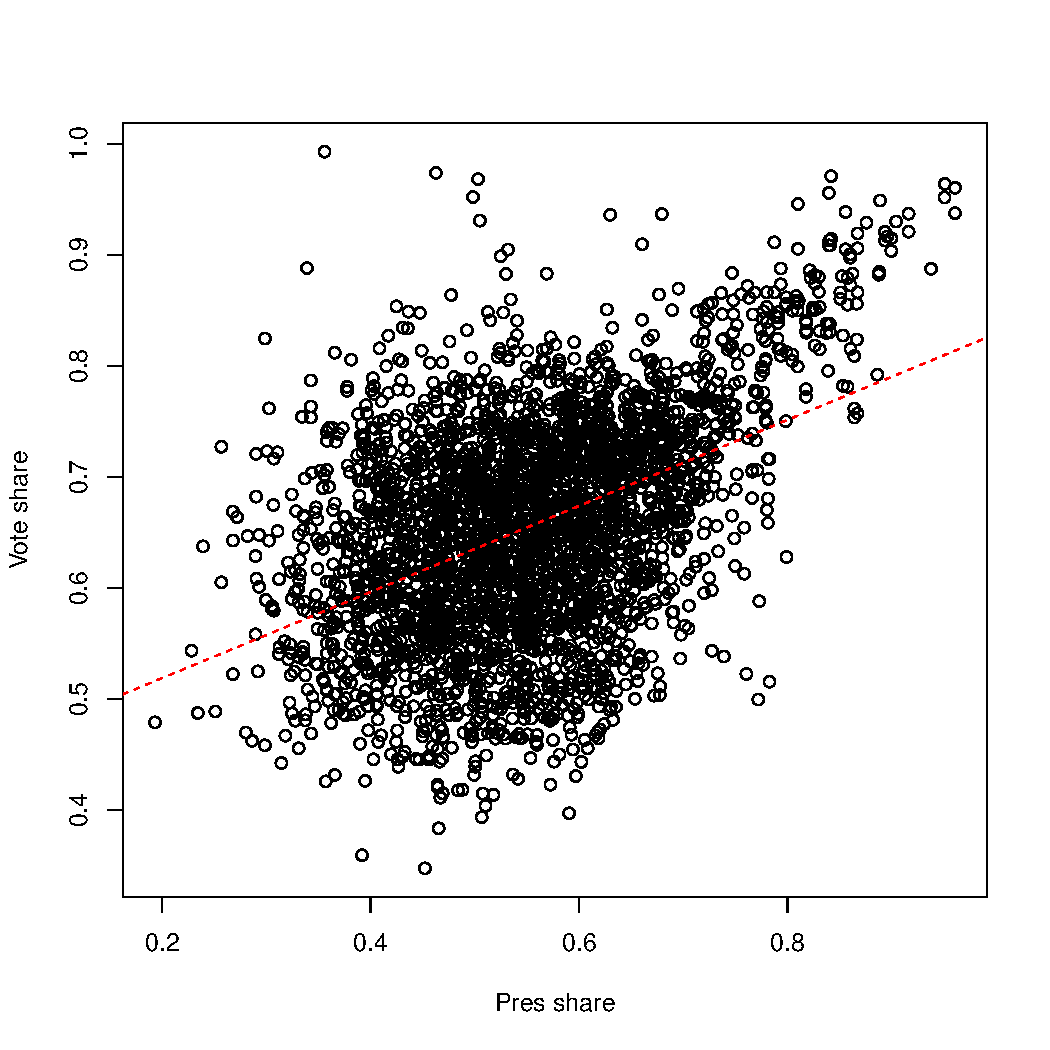
\includegraphics[width=.65\textwidth]{Q3_b.pdf}\\
\end{figure}
	\vspace{.25cm}
		\item \emph{Write the prediction equation.}
			\vspace{.25cm}
		
		
		\begin{equation*}
		voteshare = 0.441 + 0.388 \times presvote
		\end{equation*}
		
	\end{enumerate}
	
	
	\newpage	
	\section*{Question 4}
	\noindent \emph{The residuals from part (a) tell us how much of the variation in \texttt{voteshare} is $not$ explained by the difference in spending between incumbent and challenger. The residuals in part (b) tell us how much of the variation in \texttt{presvote} is $not$ explained by the difference in spending between incumbent and challenger in the district.}
	\begin{enumerate}
		\item \emph{Run a regression where the outcome variable is the residuals from Question 1 and the explanatory variable is the residuals from Question 2.}	\vspace{.25cm}
		
				\lstinputlisting[language=R, firstline=93, lastline=95]{PS3_answerKey.R} 
				
	
	\begin{table}[h!]
		\begin{center}
			\caption{\footnotesize{Outcome variable is \texttt{model\_a.resid} and the explanatory variable is \texttt{model\_b.resid}.}} 
			\begin{tabular}{l c }
				\hline
				& Model 1 \\
				\hline		
			(Intercept)    & $-0.000$      \\
			& $(0.001)$     \\
			model\_b.resid & $0.257^{***}$ \\
			& $(0.012)$     \\
			\hline
			R$^2$          & 0.130         \\
			Adj. R$^2$     & 0.130         \\
			Num. obs.      & 3193          \\
			RMSE           & 0.073         \\
				\hline
				\multicolumn{2}{l}{\scriptsize{$^{***}p<0.001$, $^{**}p<0.01$, $^*p<0.05$}}
			\end{tabular}
			
		\end{center}
	\end{table}


\noindent There is a positive and statistically reliable relationship between \texttt{model\_a.resid} and \texttt{model\_b.resid}, such that a one unit increase in the residual error from model A is associated with an average increase of 0.257 in residual error from model B (25.7\%).
	\newpage	

		\item \emph{Make a scatterplot of the two residuals and add the regression line.} 		\vspace{.25cm}
		
		\lstinputlisting[language=R, firstline=98, lastline=100]{PS3_answerKey.R}  %\newpage
		
		\begin{figure}[h!]\centering
			\caption{\footnotesize Scatter plot of \texttt{model\_a.resid} and \texttt{model\_b.resid}.}\vspace{-1cm}
			\label{fig:Q4_b}
			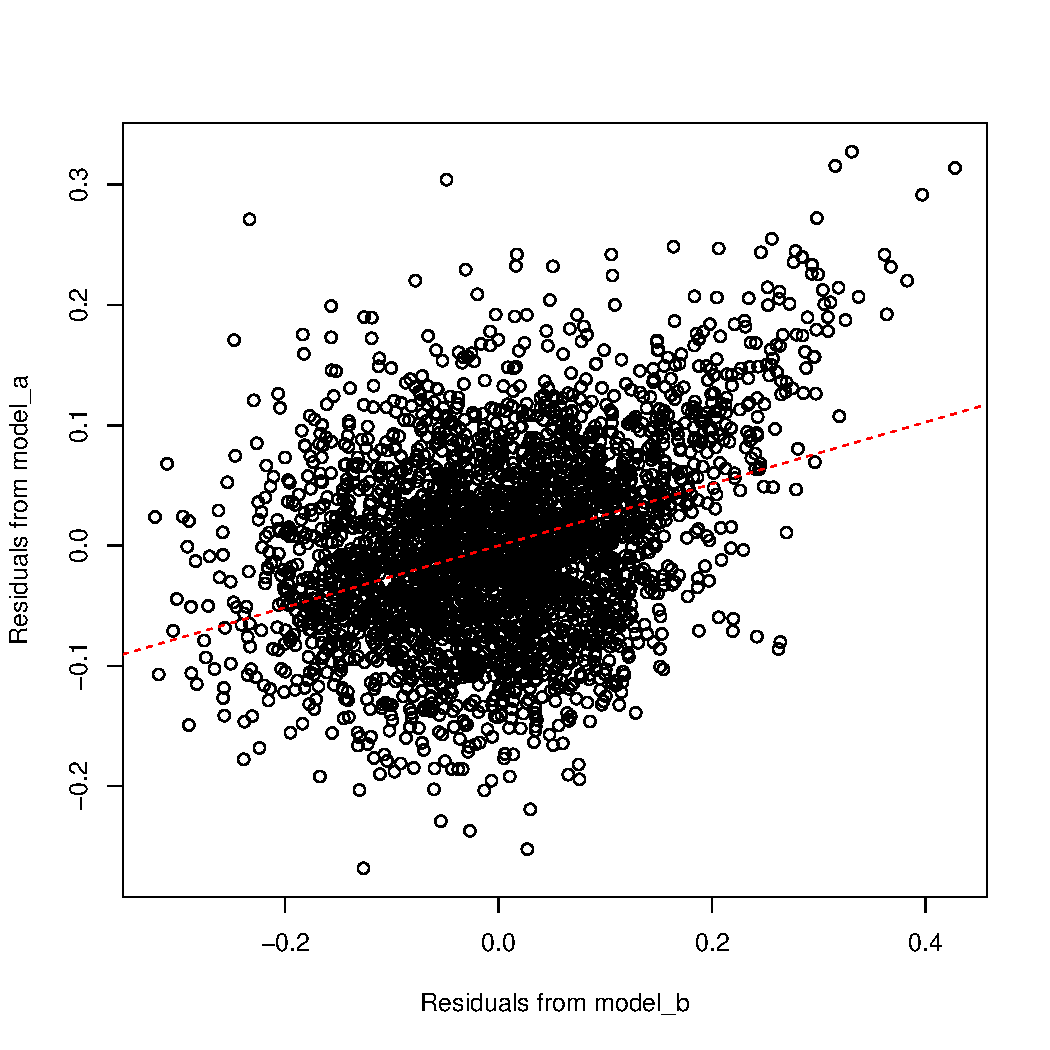
\includegraphics[width=.65\textwidth]{Q4_b.pdf}\\
		\end{figure}
\newpage
		\item \emph{Write the prediction equation.}	\vspace{.25cm}
		
		
		\begin{equation*}
		\texttt{model\_a.resid} =  0 + 0.257 \times \texttt{model\_b.resid}
		\end{equation*}
	\end{enumerate}\vspace{.25cm}
	
	\section*{Question 5}
	\noindent \emph{What if the incumbent's vote share is affected by both the president's popularity and the difference in spending between incumbent and challenger? }
	\begin{enumerate}
		\item \emph{Run a regression where the outcome variable is the incumbent's \texttt{voteshare} and the explanatory variables are \texttt{difflog} and \texttt{presvote}.}	\vspace{.25cm}
		
				\lstinputlisting[language=R, firstline=107, lastline=109]{PS3_answerKey.R}  
				
					
				\begin{table}[h!]
					\begin{center}
						\caption{\footnotesize{Outcome variable is \texttt{voteshare} and the explanatory variables are  \texttt{difflog} and \texttt{presvote}.}} 
						
						\begin{tabular}{l c }
							\hline
							& Model 1 \\
							\hline		
						(Intercept) & $0.449^{***}$ \\
            & $(0.006)$     \\
difflog     & $0.036^{***}$ \\
            & $(0.001)$     \\
presvote    & $0.257^{***}$ \\
            & $(0.012)$     \\
\hline
R$^2$       & 0.450         \\
Adj. R$^2$  & 0.449         \\
Num. obs.   & 3193          \\
RMSE        & 0.073         \\
							\hline
							\multicolumn{2}{l}{\scriptsize{$^{***}p<0.001$, $^{**}p<0.01$, $^*p<0.05$}}
						\end{tabular}
						
					\end{center}
				\end{table}
				
				\vspace{.25cm}
		\item \emph{Write the prediction equation.}	\vspace{.25cm}
		
		
		\begin{equation*}
		voteshare = 0.449 + 0.036 \times difflog + 0.257 \times presvote
		\end{equation*}
		
	\vspace{.25cm}
		
		\item \emph{What is it in this output that is identical to the output in Question 4? Why do you think this is the case?}	\vspace{.25cm}

		The coefficient for \texttt{presvote} in \texttt{model\_e} is the same as the coefficient for \texttt{model\_b.resid} in \texttt{model\_d} because it represents the partial effect of \texttt{presvote} (the amount of co-variation between \texttt{presvote} and \texttt{voteshare} that is unexplained by \texttt{difflog}).
	\end{enumerate}
	
	

\end{document}
